\documentclass[10pt, conference]{IEEEtran}
\usepackage{geometry}
\geometry{a4paper, margin=1in}
\usepackage{graphicx}
\usepackage{amsmath}
\usepackage{enumitem}
\usepackage{paracol}
\usepackage{xcolor}
\usepackage{tabularray}
\usepackage{hyperref}
\usepackage{subcaption} % Add this in the preamble

\title{
% \vspace{-2cm}
AI Project Proposal: Image Generation Using Generative AI with Minimal Objects}
\date{
% \vspace{-1cm}
\today}

\author{
    \centering
    \IEEEauthorblockN{Muhammad Hamza}
    \IEEEauthorblockA{
    `   407251 \\
        Department of Computing \\
        NUST SEECS \\
        \texttt{mhamza.bscs22seecs\\@seecs.edu.pk}
    }
    \and
    \IEEEauthorblockN{Aqsa Batool}
    \IEEEauthorblockA{
        413777 \\
        Department of Computing \\
        NUST SEECS \\
        \texttt{abatool.bscs22seecs\\@seecs.edu.pk}
    }
    \and
    \IEEEauthorblockN{Ahmed Mohiuddin Shah}
    \IEEEauthorblockA{
        415216 \\
        Department of Computing \\
        NUST SEECS \\
        \texttt{ashah.bscs22seecs\\@seecs.edu.pk}
    }
}

\begin{document}
\maketitle
\vspace{-1cm}

\section{Introduction}
The rapid advancement of Generative AI has paved the way for innovative applications in various fields, including game design and image synthesis. This project focuses on generating images using a minimal set of objects. The aim is to replicate the original image as accurately as possible while optimizing the number of objects used.

\section{Problem Identification}
Reconstructing detailed images with a limited set of objects presents a challenge in computer vision and generative algorithms. The main issue is balancing image fidelity with the number of elements used, as current methods often sacrifice computational efficiency for accuracy, or vice versa. This project aims to explore innovative generative models that maintain high image similarity while minimizing object usage.

\section{Literature Review}
Genetic algorithms (GAs) have long been celebrated for their ability to mimic evolutionary processes and adapt complex problem-solving approaches inspired by natural selection. Originating from the work of John Holland, these algorithms are rooted in mechanisms akin to biological evolution, specifically natural selection and genetic recombination \hypertarget{ref}{\textsuperscript{\hyperref[sec:1r]{[1]}\label{sec:1}}}. GAs simulate the "survival of the fittest" paradigm, where the selection, crossover, and mutation of potential solutions iteratively refine the population towards more optimal solutions \hypertarget{ref}{\textsuperscript{\hyperref[sec:2r]{[2]}\label{sec:2}}}. The foundational concepts, alongside enhancements to these processes, have been applied to diverse domains, including image reconstruction and data analysis \hypertarget{ref}{\textsuperscript{\hyperref[sec:1r]{[1]}\label{sec:1}}}.

Holland's early exploration and subsequent popularization of GAs highlighted their capability to overcome the traditional hurdles of algorithmic problem-solving by employing principles of natural selection and genetic diversity \hypertarget{ref}{\textsuperscript{\hyperref[sec:2r]{[2]}\label{sec:2}}}. His methods laid the groundwork for the algorithmic framework that would be expanded upon by later researchers \hypertarget{ref}{\textsuperscript{\hyperref[sec:3r]{[3]}\label{sec:3}}}. For instance, the classical structure of GAs involves initializing a population with potential solutions, assessing their fitness, and applying crossover and mutation operators to generate new populations. This iterative method fosters the development of solutions by combining the best traits of parent individuals \hypertarget{ref}{\textsuperscript{\hyperref[sec:3r]{[3]}\label{sec:3}}}.

Recent studies have expanded the application of GAs to image processing and artistic creation. One notable area of investigation is the use of GAs to reconstruct binary or non-photo-realistic images from random initial conditions \hypertarget{ref}{\textsuperscript{\hyperref[sec:1r]{[1]}\label{sec:1}}}\hypertarget{ref}{\textsuperscript{\hyperref[sec:5r]{[5]}\label{sec:5}}}. By using techniques such as crossover and mutation, these algorithms can generate abstract or painterly images that evolve over successive generations, providing insights into both the algorithm's creative potential and its technical limitations \hypertarget{ref}{\textsuperscript{\hyperref[sec:5r]{[5]}\label{sec:5}}}\hypertarget{ref}{\textsuperscript{\hyperref[sec:6r]{[6]}\label{sec:6}}}. This application is particularly relevant as researchers explore how genetic algorithms can go beyond traditional data processing into realms of artistic expression and visualization.

Further advancements in multi-objective genetic algorithms (MOGAs) have introduced methods to address complex optimization problems, such as recovering lost image data during compression or resizing \hypertarget{ref}{\textsuperscript{\hyperref[sec:4r]{[4]}\label{sec:4}}}. The scalability of such approaches, especially when implemented in distributed systems, highlights their practical utility in cloud computing and data transmission. These methods demonstrate how GAs can leverage parallel computing power to optimize space without compromising significant image details, thus showcasing their adaptability to real-world data processing needs \hypertarget{ref}{\textsuperscript{\hyperref[sec:4r]{[4]}\label{sec:4}}}.

Moreover, the representation of individuals within GAs has evolved over time, impacting their effectiveness in creative and computational tasks. Traditional approaches often utilized simple data structures, but recent experiments have implemented individuals as complex entities, such as arrays of RGB values, allowing for detailed image manipulations \hypertarget{ref}{\textsuperscript{\hyperref[sec:5r]{[5]}\label{sec:5}}}. This diversification in individual representation has opened up novel possibilities for evolutionary art, where genetic algorithms are harnessed to generate unique, aesthetic images that mirror the painterly styles traditionally associated with human artists \hypertarget{ref}{\textsuperscript{\hyperref[sec:6r]{[6]}\label{sec:6}}}. The success of these approaches emphasizes the potential of GAs to merge computation with creativity, demonstrating their broad applicability and versatility in solving a wide array of problems.

In summary, genetic algorithms have proven to be robust tools capable of solving highly varied and complex problems by emulating the processes of evolution. The ongoing advancements in GA methodologies, from classical representations to multi-objective optimization and artistic applications, continue to inspire further research and application across numerous fields \hypertarget{ref}{\textsuperscript{\hyperref[sec:1r]{[1]}\label{sec:1}}}\hypertarget{ref}{\textsuperscript{\hyperref[sec:2r]{[2]}\label{sec:2}}}\hypertarget{ref}{\textsuperscript{\hyperref[sec:4r]{[4]}\label{sec:4}}}\hypertarget{ref}{\textsuperscript{\hyperref[sec:5r]{[5]}\label{sec:5}}}\hypertarget{ref}{\textsuperscript{\hyperref[sec:6r]{[6]}\label{sec:6}}}. The works discussed here collectively illustrate the progression from fundamental theories of genetic algorithms to sophisticated implementations capable of generating and refining complex images, showcasing the broad scope and transformative potential of this field \hypertarget{ref}{\textsuperscript{\hyperref[sec:2r]{[2]}\label{sec:2}}}\hypertarget{ref}{\textsuperscript{\hyperref[sec:3r]{[3]}\label{sec:3}}}\hypertarget{ref}{\textsuperscript{\hyperref[sec:5r]{[5]}\label{sec:5}}}.

\section{Research Gap Identification}
While existing research highlights various generative techniques, few approaches emphasize achieving high-fidelity images using minimal objects. Most current solutions lack efficiency when applied to resource-constrained environments. We aim to introduce an optimized method for image reconstruction that ensures both accuracy and minimal object usage.

\section{Project Methodology}
Initial prototypes have been developed to test the feasibility of our approach. Early results indicate promising outcomes, where generated images closely resemble their originals with fewer objects. The next phase involves refining the model architecture and performing comprehensive evaluations to benchmark performance against current methods.

\subsection*{
Initial Test
}
We did an initial test with 10,000 generation steps on a basic model which only uses ellipses:\\
\begin{figure}[h]
    \centering
    \begin{subfigure}{0.4\linewidth}
        \centering
        
\includegraphics[width=\linewidth]{eren orig.png}
        \caption{Original Image}
    \end{subfigure}%
    \hfill
    \begin{subfigure}{0.4\linewidth}
        \centering
        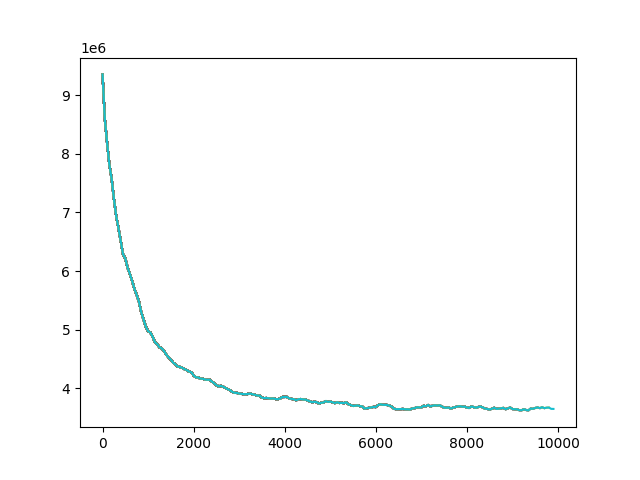
\includegraphics[width=\linewidth]{fitness_generation_9900.png}
        \caption{Fitness Graph}
    \end{subfigure}
    \begin{subfigure}{0.4\linewidth}
        \centering
        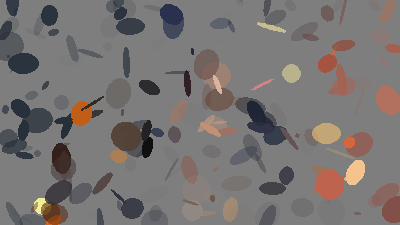
\includegraphics[width=\linewidth]{generated_100.png}
        \caption{100 generations}
    \end{subfigure}
    \begin{subfigure}{0.4\linewidth}
        \centering
        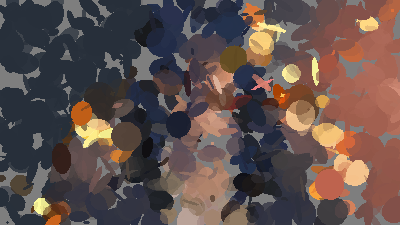
\includegraphics[width=\linewidth]{generated_9900.png}
        \caption{9900 generations}
    \end{subfigure}
    \caption{Recreating original image using basic Algoritm Implementation}
\end{figure}

Using fitness graph, we can see that our fitness has stagnated and isn't going much further.

\section{Contributions of Each Member}

\begin{enumerate}[label=\arabic*)]
    \item  Each member contributed 2 research paper each and analysed them for literature review and feasibility study.
    \item \textbf{Aqsa Batool}: Conducted literature review and analyzed existing methods focused on object constraints.
    \item \textbf{Muhammad Hamza}: Focused on comparing traditional approaches and implementing optimization techniques.
    \item \textbf{Ahmed Mohiuddin Shah}: Led prototype development and testing and analyzed hardware constraints.
\end{enumerate}

\section{References}
\begin{itemize}
    \item \textbf{\hyperref[sec:1]{[1]\label{sec:1r}}} Mirjalili, S., Song Dong, J., Sadiq, A.S., Faris, H. (2020). Genetic Algorithm: Theory, Literature Review, and Application in Image Reconstruction. In: Mirjalili, S., Song Dong, J., Lewis, A. (eds) Nature-Inspired Optimizers. Studies in Computational Intelligence, vol 811. Springer, Cham. 
    \url{https://doi.org/10.1007/978-3-030-12127-3_5}
    
    \item \textbf{\hyperref[sec:2]{[2]\label{sec:2r}}} Holland, J. H. (1992). Genetic Algorithms. Scientific American, 267(1), 66–73. \url{http://www.jstor.org/stable/24939139}
    \item \textbf{\hyperref[sec:3]{[3]\label{sec:3r}}} Genetic Algorithms
 STEPHANIE FORREST
 Department of Computer Science, University of New Mexico, Albuquerque forrest@cs.unm.edu 
 \url{https://dl.acm.org/doi/pdf/10.1145/234313.234350}
    \item \textbf{\hyperref[sec:4]{[4]\label{sec:4r}}} A Genetic Algorithm Approach to Regenerate Image from a Reduce Scaled Image Using Bit Data Count Kishor Datta Gupta Ph.D. Student, Computer Science University of Memphis, United States of America 3720 Alumni Ave, Memphis, TN 38152, USA kdgupt1@memphis.edu Sajib Sen Ph.D. Student, Computer Science University of Memphis, United States of America 3720 Alumni Ave, Memphis, TN 38152, USA ssen4@memphis.edu \url{https://lumenpublishing.com/journals/index.php/brain/article/view/2031/1688}
    
    \item \textbf{\hyperref[sec:5]{[5]\label{sec:5r}}} \url{https://github.com/SebastianCharmot/Genetic-Algorithm-Image-Recreation/blob/master/CSC_370_Final_Project_Sebastian_Daniel.pdf}
    Genetic Programming for Non-Photorealistic Image Generation
  Sebastian Charmot and Daniel Cowan 
secharmot,
dacowan@
davidson.edu
 Davidson College
 Davidson, NC 28035
 U.S.A.
 
    \item \textbf{\hyperref[sec:6]{[6]\label{sec:6r}}} Baniasadi, M., Ross, B.J. Exploring non-photorealistic rendering with genetic programming. Genet Program Evolvable Mach 16, 211–239 (2015). \url{https://doi.org/10.1007/s10710-014-9234-0}
\end{itemize}

\end{document}
